\documentclass[DaoFP]{subfiles}
\begin{document}
\setcounter{chapter}{16}

\chapter{Ends and Coends}

\section{Profunctors}

In the rarified air of category theory we encounter patterns that are so far removed from their origins that we have problems visualizing them. It doesn't help that the more abstract a pattern gets the more dissimilar the concrete examples of it are. 

An arrow from $a$ to $b$ is relatively easy to visualize. We have a very familiar model for it: a function that consumes elements of $a$ and produces elements of $b$. A hom-set is a collection of such arrows. 

A functor is an arrow between categories. It consumes objects and arrows from one category and produces objects and arrows from another. We can think of it a recipe for building such objects (and arrows) from materials provided by the source category. In particular, we  often think of an endofunctor as a container of building materials.

A profunctor maps a pair of objects $\langle a, b \rangle$ to a set $P\langle a, b \rangle$ and a pair of arrows:
\[ \langle f \colon s \to a, g \colon b \to t \rangle \]
to a function:
\[ P\langle f, g \rangle \colon P\langle a, b \rangle \to P\langle s, t \rangle\]

A profunctor is an abstraction that combines elements of many other abstractions. Since it's a functor $ \mathcal{C}^{op} \times  \mathcal{C} \to \mathbf{Set}$, we can think of it as constructing a set from a pair of objects, and a function from a pair of arrows (one of them going in the opposite direction). This doesn't help our imagination though.

Fortunately, we have a good model for a profunctor: the hom-functor. The set of arrows between two objects behaves like a profunctor when you vary the objects. It also makes sense that there is a difference between varying the source and the target of the hom-set. 

We can, therefore, think of an arbitrary profunctor as generalizing the hom-functor. A profunctor provides additional bridges between objects, on top of hom-sets that are already there. 

There is, however one big difference between an element of the hom-set $ \mathcal{C}(a, b)$ and an element of the set $P\langle a, b \rangle$. Elements of hom-sets are arrows, and arrows can be composed. It's not immediately obvious how to compose profunctors. 

Granted, the lifting of arrows by a profunctor can be seen as generalizing composition---just not between profuctors, but between hom-sets and profunctors. For instance, we can ``precompose'' $P \langle a, b \rangle$ with an arrow $f \colon s \to a$ to obtain $P \langle s, b \rangle$:
\[ P\langle f, id_b \rangle \colon P \langle a, b \rangle \to P \langle s, b \rangle \]
Similarly, we can ``postcompose'' it with $g \colon b \to t$:
\[ P \langle id_a, g \rangle \colon P \langle a, b \rangle \to P \langle a, t \rangle \]
This kind of heterogenous composition takes a composable pair consisting of an arrow and an element of a profunctor and produces an element of a profunctor.

A profunctor can be extended this way on both sides by lifting a pair of arrows:

\[
 \begin{tikzcd}
  & s
  \arrow[r, bend left, dashed, blue, "f"]
 & a
 \arrow[r, bend right, "P"]
 & b
  \arrow[r, bend left, dashed, blue, "g"]
 &  t
  \end{tikzcd}
\]

\subsection{Collages}

There is no reason to restrict a profunctor to a single category. We can easily define a profunctor between two categories as a functor $ P \colon \mathcal{C}^{op} \times  \mathcal{D} \to \mathbf{Set}$. Such a profunctor can be used to glue two categories together by generating the missing hom-sets from the objects in $\mathcal{C}$ to the objects in $\mathcal{D}$. 

A collage (or a \index{cograph}cograph) of two categories $\mathcal{C}$ and $\mathcal{D}$ is a category whose objects are objects from both categories (a disjoint union). A hom-set between two objects $x$ and $y$ is either a hom-set in $\mathcal{C}$, if both objects are in $\mathcal{C}$; a hom-set in $\mathcal{D}$, if both are in $\mathcal{D}$; or the set $P \langle x, y\rangle$ if $x$ is in $\mathcal{C}$ and $y$ is in $\mathcal{D}$. Otherwise the hom-set is empty. 

Composition of morphisms is the usual composition, except if one of the morphisms is an element of $P \langle x, y \rangle$. In that case we lift the morphism we're trying to pre- or post-compose. 

It's easy to see that a collage is indeed a category. The new morphisms that go between the two sides of the collage are sometimes called \index{heteromorphism}heteromorphisms. They can only go from $\mathcal{C}$ to $\mathcal{D}$, never the other way around. 

Seen this way, a profunctor $ \mathcal{C}^{op} \times  \mathcal{C} \to \mathbf{Set}$ should really be called an \emph{endo}-profunctor. It defines a collage of $\mathcal{C}$ with itself.

\begin{exercise}
Show that there is a functor from a collage of two categories to a stick-figure ``walking arrow'' category that has two objects and one arrow between them (and two identity arrows).
\end{exercise}
\begin{exercise}
Show that, if there is a functor from $\mathcal{C}$ to the walking arrow category then $\mathcal{C}$ can be split into a collage of two categories. 
\end{exercise}

\subsection{Profunctors as relations}

Under a microscope, a profunctor looks like a hom-functor, and the elements of the set $P \langle a, b \rangle$ look like individual arrows. But when we zoom out, we can view a profunctor as a relation between objects. These are not the usual relations; they are \index{proof-relevant relation}\emph{proof-relevant} relations.

To understand this concept better, let's consider a regular functor $F \colon \mathcal{C} \to \mathbf{Set}$ (in other words, a co-presheaf). One way to interpret it is to say that it definines a \index{proof-relevant subset} subset of objects of $\mathcal{C}$, namely those objects that are mapped to non-empty sets. Every element of $F a$ is then treated as a proof that $a$ is a member of this subset. If, on the other hand, $F a$ is an empty set, then $a$ is not a member of the subset.

We can apply the same interpretation to profunctors. If the set $P \langle a, b \rangle$ is empty, we say that $b$ is not related to $a$. If it's not empty, we say that each element of the set $P \langle a, b \rangle$ represents a proof that $b$ is related to $a$. We can then treat a profunctor as a proof-relevant relation. 

Notice that we don't assume anything about this relation. It doesn't have to be reflexive, as it's possible for $P \langle a, a \rangle$ to be empty (in fact, $P \langle a, a \rangle$ makes sense only for endo-profunctors). It doesn't have to be symmetric either.

Since the hom-functor is an example of an (endo-) profunctor, this interpretation lets us view the hom-functor in a new light: as a built-in proof-relevant relation between objects in a category. If there's an arrow between two objects, they are related. Notice that this relation is reflexive, since $\mathcal{C}(a, a)$ is never empty: at the very least, it contains the identity morphism. 

Moreover, as we've seen before, hom-functors interact with profunctors. If $a$ is related to $b$ through $P$, and the hom-sets $\mathcal{C}(s, a)$ and $\mathcal{D}(b, t)$ are non-empty, then automatically $s$ is related to $t$ through $P$. Profunctors are therefore proof-relevant relations that are compatible with the structure of the categories in which they operate.

We know how to compose a profunctor with hom-functors, but how would we compose two profunctors? We can get a clue from the composition of relations. 

Suppose that you want to charge your cellphone, but you don't have a charger. In order to connect you to a charger it's enough that you have a friend who owns a charger. Any friend will do. You compose the relation of having a friend with the relation of a person having a charger to get a relation of being able to charge your phone. The proof that you can charge your phone is a pair of proofs, one of friendship and one of the possession of a charger. 

In general, we say that two objects are related by the composite relation if there exists an object in the middle that is related to both of them. 

\subsection{Profunctor composition in Haskell}

Composition of relations can be translated to profunctor composition in Haskell. Let's first recall the definition of a profunctor:
\begin{haskell}
class Profunctor p where
  dimap :: (s -> a) -> (b -> t) -> (p a b -> p s t)
\end{haskell}

The key to understanding profunctor composition is that it requires the \emph{existence} of the object in the middle. For object $b$ to be related to object $a$ through the composite $P \diamond Q$ there has to exist an object $x$ that bridges the gap:
\[
 \begin{tikzcd}
  & a
  \arrow[r, bend left, blue, "Q"]
 & x
  \arrow[r, bend left, red, "P"]
 & b
  \end{tikzcd}
\]

This can be encoded in Haskell using an existential type. Given two profunctors \hask{p} and \hask{q}, their composition is a new profunctor \hask{Procompose p q}:
\begin{haskell}
data Procompose p q a b where
  Procompose ::  q a x -> p x b -> Procompose p q a b
\end{haskell}
We are using a \hask{GADT} to express the existential nature of the object \hask{x}. The two arguments to the data constructor can be seen as a pair of proofs: one proves that \hask{x} is related to \hask{a}, and the other that \hask{b} is related to \hask{x}. This pair then constitutes the proof that \hask{b} is related to \hask{a}.

An existential type can be seen as a generalization of a sum type. We are summing over all possible types \hask{x}. Just like a finite sum can be constructed by injecting one of the alternatives (think of the two constructors of \hask{Either}), the existential type can be constructed by picking one particular type for \hask{x} and injecting it into the definition of \hask{Procompose}. 

Just as mapping out from a sum type requires a pair of function, one per each alternative; a mapping out from an existential type requires a family of functions, one per every type. The mapping out from \hask{Procompose}, for instance, is given by a polymorphic function:
\begin{haskell}
mapOut :: Procompose p q a b -> (forall x. q a x -> p x b -> c) -> c
mapOut (Procompose qax pxb) f = (f qax pxb)
\end{haskell}

The composition of profunctors is again a profunctor, as can be seen from this instance:
\begin{haskell}
instance (Profunctor p, Profunctor q) => Profunctor (Procompose p q) 
  where
    dimap l r (Procompose qax pxb) = 
               Procompose (dimap l id qax) (dimap id r pxb)
\end{haskell}
This is just saying that you can extend the composite profunctor by extending the first one to the left and the second one to the right.

The fact that this definition of profunctor composition happens to work in Haskell is due to parametricity. The language constraints the types of profunctors in a way that makes this work. In general, though, taking a simple sum over intermediate objects would result in over-counting, so in category theory we have to compensate for that.

\section{Coends}

The over-counting in the naive definition of profunctor composition happens when two candidates for the object in the middle are connected by a morphism:
\[
 \begin{tikzcd}
  & a
  \arrow[r, bend left, blue, "Q"]
  &x
  \arrow[r, dashed, "f"]
 & y
  \arrow[r, bend left, red, "P"]
 & b
  \end{tikzcd}
\]
We can either extend $Q$ on the right, by lifting $Q \langle id, f \rangle$, and use $y$ as the middle object; or we can extend $P$ on the left, by lifting $P \langle f, id \rangle$, and use $x$ as the intermediary.

In order to avoid the double-counting, we have to tweak our definition of a sum type when applied to profunctors. The resulting construction is called a coend. 

First, let's re-formulate the problem. We are trying to sum over all objects $x$ in the product:
\[ P \langle a, x \rangle \times Q \langle x, b \rangle \]
The double-counting happens because we can open up the gap between the two profunctors, as long as there is a morphism that we can fit between them. So we are really looking at a more general product:
\[ P \langle a, x \rangle \times Q \langle y, b \rangle \]
The important observation is that, if we fix the endpoints $a$ and $b$, this product is a profunctor in $\langle y, x \rangle$. This is easily seen after a little rearrangement (up to isomorphism):
\[ Q \langle y, b \rangle \times P \langle a, x \rangle \]
We are interested in the sum of the diagonal parts of this profunctor, that is when $x$ is equal to $y$. 

So let's see how we would go about defining the sum of all diagonal entries of a general profunctor $P$. In fact, this construction works for any functor $P \colon \cat C^{op} \times \cat C \to D$, not just for $\Set$-valued profunctors. 

The sum of the diagonal objects is defined by injections; in this case, one per every object in $\cat C$. Here we show just two of them and the dashed line representing all the rest:
\[
 \begin{tikzcd}
 P \langle y, y \rangle
 \arrow[dr, "i_y"']
 \arrow[rr, dash, dashed]
 &&P \langle x, x \rangle
 \arrow[dl, "i_x"]
 \\
 & d
 \end{tikzcd}
\]

If we were defining a sum, we'd make it a universal object equipped with such injections. But because we are dealing with functors of two variables, we want to identify the injections that are related by ``extending'' some common ancestor (here, $P \langle y, x \rangle$). We want the following diagram to commute, whenever there is a connecting morphism $f\colon x \to y$:

\[
 \begin{tikzcd}
 &P \langle y, x \rangle
 \arrow[ld, "{P \langle id, f \rangle}"']
 \arrow[rd, "{P \langle f, id \rangle}"]
 \\
 P \langle y, y \rangle
 \arrow[dr, "i_y"']
 &&P \langle x, x \rangle
 \arrow[dl, "i_x"]
 \\
 &d
 \end{tikzcd}
\]
This diagram is called a \index{co-wedge}co-wedge, and its commuting condition is called the co-wedge condition. For every $f \colon x \to y$, we demand that:
\[ i_x \circ P \langle f, id_y \rangle = i_y \circ P \langle id_x, f \rangle \]
The \emph{universal} co-wedge is called a coend.

Since a coend generalizes the sum to a potentially infinite domain, we write it using the integral sign, with the ``integration variable'' at the top:
\[ \int^{x\colon \mathcal{C}} P \langle x, x \rangle \]
Universality means that, whenever there is an object $d$ in $\cat D$ equipped with a family of arrows $g_x \colon P \langle x, x \rangle \to d$ satisfying the co-wedge condition, there is a unique mapping out from the coend:
\[ h \colon \int^{x\colon \mathcal{C}} P \langle x, x \rangle \to d \]
that factorizes every $g_x$ through the injection $i_x$:
\[ g_x = h \circ i_x \]
Pictorially, we have:
\[
 \begin{tikzcd}
 &P \langle y, x \rangle
 \arrow[ld, "{P \langle id, f \rangle}"']
 \arrow[rd, "{P \langle f, id \rangle}"]
 \\
 P \langle y, y \rangle
 \arrow[dr, "i_y"']
 \arrow[ddr, bend right,  "g_y"']
 &&P \langle x, x \rangle
 \arrow[dl, "i_x"]
 \arrow[ddl, bend left,  "g_x"]
 \\
 &\int^x P \langle x, x \rangle
 \arrow[d, dashed, "h"]
 \\
 &d
 \end{tikzcd}
\]

Compare this with the definition of a sum of two objects:

\[
 \begin{tikzcd}
 a
 \arrow[dr, "\text{Left}"]
 \arrow[ddr, bend right, "f"']
 && b
 \arrow[dl, "\text{Right}"']
 \arrow[ddl, bend left, "g"]
 \\
&a + b
\arrow[d, dashed, "h"]
\\
& d
 \end{tikzcd}
\]
Just like the sum was defined as a universal cospan, a coend is defined as a universal co-wedge. 

In particular, if you were to construct a coend of a $\Set$-valued profunctor, you would start with a sum (a discriminated union) of all the sets $P \langle x, x \rangle$. Then you would identify all the elements of this sum that satisfy the co-wedge condition. You'd identify the element $a \in P \langle x, x \rangle$ with the element $b \in P \langle y, y \rangle$ whenever there is an element $c  \in P \langle y, x \rangle$ and a morphism $f \colon x \to y$, such that:
\[ P \langle id, f \rangle (c) = b\]
and
\[ P \langle f, id \rangle (c) = a\]

Notice that, in a discrete category (which is just a set of objects with no arrows between them) the co-wedge condition is trivial (there are no $f$'s other than identities), so a coend is just a straightforward sum (coproduct) of the diagonal objects $P \langle x, x \rangle$.

\subsection{Extranatural transformations}

A family of arrows in the target category parameterized by the objects of the source category can often be combined into a single natural transformation between two functors. 

The injections in our definition of a cowedge form a family of functions that is parameterized by objects, but they don't neatly fit into a definition of a natural transformation.
\[
 \begin{tikzcd}
 P \langle y, y \rangle
 \arrow[dr, "i_y"']
 \arrow[rr, dash, dashed]
 &&P \langle x, x \rangle
 \arrow[dl, "i_x"]
 \\
 &d
 \end{tikzcd}
\]
The problem is that the functor $P \colon \cat C^{op} \times \cat C \to \cat D$ is contravariant in the first argument and covariant in the second; so its diagonal part, which on objects is defined as $x \mapsto P \langle x, x \rangle$, is neither.

The closest analog of naturality at our disposal is the cowedge condition:
\[
 \begin{tikzcd}
 &P \langle y, x \rangle
 \arrow[ld, "{P \langle id, f \rangle}"']
 \arrow[rd, "{P \langle f, id \rangle}"]
 \\
 P \langle y, y \rangle
 \arrow[dr, "i_y"']
 &&P \langle x, x \rangle
 \arrow[dl, "i_x"]
 \\
 &d
 \end{tikzcd}
\]
Indeed, as is the case with the naturality square, it involves the interaction between the lifting of a morphism $f \colon x \to y$ (here, in two different ways) and the components of the transformation $i$. 

Granted, the standard naturality condition deals with pairs of functors. Here, the target of the transformation is a fixed object $d$. But we can always reinterpret it as the output of a constant functor $\Delta_d \colon \cat C^{op} \times \cat C \to \cat D$.

The cowedge condition can be interpreted as a special case of the more general \index{extranatural transformation}\emph{extranatural} transformation. An extranatural transformation is a family of arrows:
\[ \alpha_{c d} \colon P \langle c, c \rangle \to Q \langle d, d \rangle \]
between two functors of the form:
\[ P \colon \cat C^{op} \times \cat C \to \cat E \]
\[ Q \colon \cat D^{op} \times \cat D \to \cat E \]
Extranaturality in $c$ means that the following diagram commutes for any morphism $f \colon c \to c'$:
\[
 \begin{tikzcd}
 &P \langle c', c \rangle
 \arrow[ld, "{P \langle id, f \rangle}"']
 \arrow[rd, "{P \langle f, id \rangle}"]
 \\
      P \langle c', c' \rangle
 \arrow[dr, "\alpha_{c' d}"']
 &&P \langle c, c \rangle
 \arrow[dl, "\alpha_{c d}"]
 \\
 & Q \langle d, d \rangle
 \end{tikzcd}
\]
Extranaturality in $d$ means that the following diagram commutes for any morphism $g \colon d \to d'$:
\[
 \begin{tikzcd}
 &P \langle c, c \rangle
 \arrow[ld, "\alpha_{c d}"']
 \arrow[rd, "\alpha_{c d'}"]
 \\
      Q \langle d, d \rangle
 \arrow[dr, "{Q \langle id, g\rangle}"']
 &&Q \langle d', d' \rangle
 \arrow[dl, "{Q \langle g,  id\rangle}"]
 \\
 & Q \langle d, d' \rangle
 \end{tikzcd}
\]

Given this definition, we get our cowedge condition as the extranaturality of the mapping between the profunctor $P$ and the constant profunctor $\Delta_d$. 

We can now reformulate the definition of the coend as a pair $(e, i)$ where $e$ is the object equipped with the extranatural transformation  $i \colon P \to \Delta_e$ that is universal among such pairs.

Universality means that for any object $d$ equipped with the extranatural transformation $\alpha \colon P \to \Delta_d$ there is a unique morphism $h \colon e \to d$ that factorizes all the components of $\alpha$ through the components of $i$:
\[ \alpha_x = h \circ i_x \]
We call this object $e$ the coend, and write it as:
\[ e = \int^x P\langle x, x \rangle \]

\subsection{Profunctor composition using coends}

Equipped with the definition of a coend we can now formally define the composition of two profunctors:

\[ (P \diamond Q)\langle a, b \rangle = \int^{x\colon \mathcal{C}} Q \langle a, x \rangle \times P \langle x, b \rangle\]
Compare this with:
\begin{haskell}
data Procompose p q a b where
  Procompose ::  q a x -> p x b -> Procompose p q a b
\end{haskell}

The reason why in Haskell we don't have to worry about the co-wedge condition is analogous to the reason why all parametrically polymorphic functions automatically satisfy naturality condition. A coend is defined using a family of injections; in Haskell all these injections are defined by a single polymorphic function:
\begin{haskell}
data Coend p where
  Coend ::  p x x -> Coend p
\end{haskell}

Coends introduce a new level of abstraction in dealing with profunctors. Calculations using coends usually take advantage of their mapping-out property. To define a mapping out of a coend to some object $d$:
\[ \int^x P \langle x, x \rangle \to d \]
 it's enough to define a family of functions from the diagonal entries of the functor to $d$:
 \[ g_x \colon P \langle x, x \rangle \to d \]
 satisfying the cowedge condition. You can get a lot of mileage from this trick, especially when combined with the Yoneda lemma. We'll see examples of this in what follows.

\begin{exercise}
Define a \hask{Profunctor} instance for the pair of profunctors:
\begin{haskell}
newtype ProPair q p a b x y = ProPair (q a y, p x b)
\end{haskell}
Hint: Keep the first four parameters fixed:
\begin{haskell}
instance (Profunctor p, Profunctor q) => Profunctor (ProPair q p a b)
\end{haskell}
\end{exercise}

\begin{exercise}
Profunctor composition can be expressed using a coend:
\begin{haskell}
newtype CoEndCompose p q a b = CoEndCompose (Coend (ProPair q p a b))
\end{haskell}
Define a \hask{Profunctor} instance for \hask{CoEndCompose}.
\end{exercise}

\subsection{Colimits as coends}
A function of two variables that ignores one of its arguments is equivalent to a function of one variable. Similarly, a profunctor that ignores one of its arguments is equivalent to a functor. Conversely, given a functor $F$, we can construct a profunctor:
\[P \langle x, y \rangle = F y \]
Similarly, its action on a pair of arrows ignores one of the arrows:
\[P \langle f, g \rangle = F g \]
For any   $f \colon x \to y$, our definition of a coend for such a profunctor reduces to the following diagram:
\[
 \begin{tikzcd}
 & F x
 \arrow[ld, "F f"']
 \arrow[rd, dashed, "id_{F x}"]
 \\
 F y
 \arrow[dr, "i_y"']
 \arrow[ddr, bend right,  "g_y"']
 && F x
 \arrow[dl, "i_x"]
 \arrow[ddl, bend left,  "g_x"]
 \\
 &\int^x F x
 \arrow[d, dashed, "h"]
 \\
 &d
 \end{tikzcd}
\]
After shrinking the identity arrows, the original co-wedge becomes a co-cone, and the universal condition turns into the definition of a colimit. This justifies the use the coend notation for colimits:
\[ \int^x F x = \text{colim} F \]
The functor $F$ defines a diagram in the target category. The source category, in this case, is the pattern.

We can gain a useful intuition if we consider a discrete category, in which a profunctor is a (possibly infinite) matrix and a coend is the sum (coproduct) if its diagonal elements. A profunctor that is constant along one axis corresponds to a matrix whose rows are identical (each given by a ``vector'' $F x$). The sum of the diagonal elements of such a matrix is equal to the sum of all components of the vector $F x$.
\[
\begin{pmatrix}
\color{red} F a & F b & F c & ... \\
F a & \color{red}F b & F c & ...\\
F a & F b &\color{red}F c & ...\\
... & ... & ... & ...
\end{pmatrix}
\]
In a non-discrete category, this sum generalizes to a colimit.
\section{Ends}

Just like a coend generalizes a sum of the diagonal elements of a profunctor---its dual, an end, generalizes the product. A product is defined by its projections, and so is an end. 

The generalization of a span that we used in the definition of a product would be an object $d$ with a family of projections, one per every object $x$:
\[ \pi_x \colon d \to P \langle x, x \rangle \]
The dual to a co-wedge is called a \index{wedge}wedge:
\[
 \begin{tikzcd}
 &d
 \arrow[ld, "\pi_x"']
 \arrow[rd, "\pi_y"]
 \\
 P \langle x, x \rangle
 \arrow[dr, "{P \langle id, f \rangle}"']
 &&P \langle y, y \rangle
 \arrow[dl, "{P \langle f, id \rangle}"]
 \\
 & P \langle x, y \rangle
 \end{tikzcd}
\]
For every arrow $f \colon x \to y$ we demand that:
\[ P \langle f, id_y \rangle \circ \pi_y = P \langle id_x, f \rangle \circ \pi_x \]

The end is a universal wedge. We use the integral sign for it too, this time with the ``integration variable'' at the bottom. 
\[ \int_{x \colon \cat C} P \langle x, x \rangle \]

You might be wondering why integrals based on multiplication rather than summation are rarely used in calculus. That's because we can use a logarithm to replace multiplication with addition. We don't have this luxury in category theory, so ends and coends are equally important.

To summarize, an end is an object equipped with a family of morphisms (projections):
\[ \pi_a \colon \left( \int_x P \langle x, x \rangle \right) \to P \langle a, a \rangle \]
satisfying the wedge condition. 

It is universal among such objects; that is, for any other object $d$ equipped with a family of arrows $g_x$ satisfying the wedge condition, there is a unique morphism $h$ that factorizes the family $g_x$ through the family $\pi_x$:
\[ g_x = \pi_x \circ h \]
Pictorially, we have:
\[
 \begin{tikzcd}
 &d
 \arrow[ddl, bend right, "g_x"']
 \arrow[ddr, bend left, "g_y"]
 \arrow[d, dashed, "h"]
 \\
 & \int_x P \langle x, x \rangle
 \arrow[ld, "\pi_x"']
 \arrow[rd, "\pi_y"]
 \\
 P \langle x, x \rangle
 \arrow[dr, "{P \langle id, f \rangle}"']
 &&P \langle y, y \rangle
 \arrow[dl, "{P \langle f, id \rangle}"]
 \\
 & P \langle x, y \rangle
 \end{tikzcd}
\]

Equivalently, we can say that the end is a pair $(e, \pi)$ consisting of an object $e$ and an  extranatural transformation $\pi \colon \Delta_d \to e$ that is universal among such pairs. The wedge condition turns out to be a special case of extranaturality condition.

If you were to construct an end of a $\Set$-valued profunctor, you'd start with a product of all $P \langle x, x \rangle$ for all objects in the category and then prune the tuples that don't satisfy the wedge condition. 

In particular, imagine using the singleton set $1$ in place of $d$. The family $g_x$ would select one element from each set $P \langle x, x \rangle$. This would give you a giant tuple. You'd weed out most of these tuples, leaving only the ones that satisfy the wedge condition. 

Again, in Haskell, due to parametricity, the wedge condition is automatically satisfied, and the definition of an end for a profunctor \hask{p} simplifies to:

\begin{haskell}
type End p = forall x. p x x
\end{haskell}

The Haskell implementation of an \hask{End} doesn't showcase the fact that it is dual to the \hask{Coend}. This is because, at the time of this writing, Haskell doesn't have a built-in syntax for existential types. If it did, the \hask{Coend} would be implemented as:
\begin{haskell}
type Coend p = exists x. p x x
\end{haskell}

The existential/universal duality between a \hask{Coend} and an \hask{End} means that it's easy to construct a \hask{Coend}---all you need is to pick one type \hask{x} for which you have a value of the type \hask{p x x}. On the other end, to construct an \hask{End} you have to provide a whole family of values \hask{p x x}, one for every type \hask{x}. In other words, you need a polymorphic formula that is parameterized by \hask{x}. A definition of a polymorphic function is a canonical example of such a formula.


\subsection{Natural transformations as an end}

The most interesting application of an end is in concisely defining natural transformations. Consider two functors, $F$ and $G$, going between two categories  $\mathcal{B}$ and $\mathcal{C}$. A natural transformation between them is a family of arrows $\alpha_x$ in $\mathcal{C}$. You may think of it as picking one element $\alpha_x$ from each hom-set  $\mathcal{C} (F x, G x)$.
\[
 \begin{tikzcd}
 && F x
 \arrow[dd, "\alpha_x"]
 \\
 x
 \arrow[urr, dashed, "F"]
 \arrow[drr, dashed, "G"]
 \\
 && G x
 \end{tikzcd}
\]

We know that the mapping $\langle a, b \rangle \to \mathcal{C} (a, b)$ defines a profunctor.  It turns out that, for any pair of functors, the mapping  $\langle a, b \rangle \to \mathcal{C} (F a, G b)$ also behaves like a profunctor. Its action on a pair of arrows $\langle f, g \rangle$ is a combination of pre- and post-composition of lifted arrows:
 \[ (G g) \circ - \circ (F f) \]

Indeed, an element of the set $ \mathcal{C} (F a, G b)$ is an arrow $h \colon F a \to G b$. We are trying to lift a pair of arrows $f \colon s \to a$ and $g \colon b \to t$. We can do it with a pair of arrows in $\mathcal{C}$: the first one is $F f \colon F s \to F a$, and the second one is $G g \colon G b \to G t$. The composition $G g \circ h \circ F f$ gives us the desired result $ F s \to G t$, which is an element of $\mathcal{C} (F s, G t)$.
\[ F s \xrightarrow{F f} F a \xrightarrow{h} G b \xrightarrow{G g} G t \]

The diagonal parts of this profunctor are good candidates for the components of a natural transformation. In fact, the end:
\[  \int_{x \colon  \mathcal{B}} \mathcal{C}(F x, G x) \]
defines a set of natural transformations from $F$ to $G$.

In Haskell, this is consistent with our earlier definition:
\begin{haskell}
type Natural f g = forall x. f x -> g x
\end{haskell}

In category theory, though, we have to check the wedge condition. Plugging in our profunctor, we get:

\[
 \begin{tikzcd}
 & \int_{x} \mathcal{C}(F x, G x)
 \arrow[ld, "\pi_a"']
 \arrow[rd, "\pi_b"]
 \\
  \mathcal{C} ( F a, G a )
 \arrow[dr, "{(Ff \, \circ \, -)}"']
 && \mathcal{C} \langle F b, G b \rangle
 \arrow[dl, "{(- \, \circ\, Gf)}"]
 \\
 &  \mathcal{C} ( F a, G b )
 \end{tikzcd}
\]

We can focus on a single element of the set $\int_{x} \mathcal{C}(F x, G x)$ by instantiating the universal condition for the singleton set:

\[
 \begin{tikzcd}
 & 1
 \arrow[d, dashed, "\alpha"]
\arrow[ddl, bend right, "\alpha_a"']
 \arrow[ddr, bend left, "\alpha_b"]
 \\
 & \int_{x} \mathcal{C}(F x, G x)
 \arrow[ld, "\pi_a"']
 \arrow[rd, "\pi_b"]
 \\
  \mathcal{C} ( F a, G a )
 \arrow[dr, "{(F f \, \circ \, -)}"']
 && \mathcal{C} \langle F b, G b \rangle
 \arrow[dl, "{(- \, \circ\, G f)}"]
 \\
 &  \mathcal{C} ( F a, G b )
 \end{tikzcd}
\]
It picks the component $\alpha_a$ from the hom-set $\mathcal{C} ( F a, G a )$ and the component $\alpha_b$ from $\mathcal{C} ( F b, G b )$. The wedge condition then boils down to:
\[ F f \circ \alpha_a = \alpha_b \circ G f \]
for any $f \colon a \to b$. This is exactly the naturality condition. So an element $\alpha$ of this end is indeed a natural transformation.

The set of natural transformations, or the hom-set in the functor category, is thus given by the end:
\[ [\mathcal{C}, \mathcal{D}] (F, G) \cong \int_{x \colon  \mathcal{B}} \mathcal{C}(F x, G x)\]

As we discussed earlier, to construct an \hask{End} we have to give it a whole family of values parameterized by types. Here, these values are the components of a polymorphic function. 

\subsection{Limits as ends}
Just like we were able to express colimits as coends, we can express limits as ends. As before, we define a profunctor that ignores its first argument:
\begin{align*}
 P \langle x, y \rangle &= F y \\
 P \langle f, g \rangle &= F g 
\end{align*}
The universal condition that defines an end becomes the definition of a universal cone:
\[
 \begin{tikzcd}
 &d
 \arrow[ddl, bend right, "g_x"']
 \arrow[ddr, bend left, "g_y"]
 \arrow[d, dashed, "h"]
 \\
 & \int_x F x
 \arrow[ld, "\pi_x"']
 \arrow[rd, "\pi_y"]
 \\
 F x
 \arrow[dr, "F f"']
 &&F y
 \arrow[dl, dashed, "id_{F y}"]
 \\
 & F y
 \end{tikzcd}
\]
We can thus use the end notation for limits:
\[ \int_x F x = \text{lim} F \]

\section{Continuity of the Hom-Functor}

In category theory, a functor is called continuous if it preserves limits (and co-continuous, if it preserves colimits). It means that, if you have a diagram in the source category then it doesn't matter if you first use the functor to map the diagram, and then take the limit; or take the limit in the source category, and use the functor to map this limit. 

The hom-functor is an example of a functor that is continuous in its second argument. Since a product is the simplest example of a limit, this means, in particular, that:
\[ \mathcal{C}(x, a \times b) \cong \mathcal{C}(x, a) \times \mathcal{C}(x, b) \]
The left hand side applies the hom-functor to the product (a limit of a span). The right hand side maps the diagram, here just a pair of objects, and takes the product (limit) in the target category. The target category for the hom-functor is $\mathbf{Set}$, so this is just a cartesian product. The two sides are isomorphic by the universal property of the product: the mapping into the product is defined by a pair of mappings into the two objects. 

Continuity of the hom-functor in the first argument is reversed: it maps colimits to limits. Again, the simplest example of a colimit is the sum, so we have:
\[ \mathcal{C}(a + b, x) \cong \mathcal{C}(a, x) \times \mathcal{C}(b, x) \]
This follows from the universality of the sum: a mapping out of the sum is defined by a pair of mapping out of the two objects.

It can be shown that an end can be expressed as a limit, and a coend as a colimit. Therefore, by continuity of the hom-functor, we can always pull out the integral sign from inside a hom-set. By analogy with the product, we have the mapping-in formula for an end:
\[\cat D\left(d, \int_a P\langle a, a \rangle \right) \cong \int_a \cat D(d, P\langle a, a \rangle) \]
By analogy with the sum, we have a mapping-out formula for the coend:
\[\cat D\left( \int^a P\langle a, a \rangle , d \right) \cong \int_a \cat D(P\langle a, a \rangle, d) \]
Notice that, in both cases, the right-hand side is an end.

\section{Fubini Rule}

The Fubini rule in calculus states the conditions under which we can switch the order of integration in double integrals. It turns out that we can similarly switch the order of double ends and coends. The Fubini rule for ends works for functors of the form $P \colon \cat C \times \cat C^{op} \times \cat D \times \cat D^{op} \to \cat E$. The following expressions, as long as they exist, are isomorphic:
\[ \int_{c \colon \cat C} \int_{d \colon \cat D} P\langle c, c \rangle \langle d, d \rangle \cong  \int_{d \colon \cat D} \int_{c \colon \cat C} P\langle c, c \rangle \langle d, d \rangle \cong  \int_{\langle c, d \rangle \colon \cat C \times \cat D}  P\langle c, c \rangle \langle d, d \rangle \]
In the last end, the funtor $P$ is reinterpreted as $P \colon (\cat C  \times \cat D)^{op} \times (\cat C \times \cat D)\to \cat E$

The analogous rule works for coends as well.

\section{Ninja Yoneda Lemma}

Having expressed the set of natural transformations as an end, we can now rewrite the Yoneda lemma. This is the original formulation:
\[ [\mathcal{C}, \mathbf{Set}]( \mathcal{C}(a, -), F) \cong F a \]
Here, $F$ is a (covariant) functor from $\mathcal{C}$ to $\mathbf{Set}$ (a co-presheaf), and so is the hom-functor $\mathcal{C}(a, -)$. 
Expressing the set of natural transformations as an end we get:
\[ \int_{x \colon \mathcal{C}} \mathbf{Set} (\mathcal{C}(a, x), F x) \cong F a \]

Similarly, we have the Yoneda lemma for a contravariant functor (a presheaf) $G$:
\[ \int_{x \colon \mathcal{C}} \mathbf{Set} (\mathcal{C}(x, a), G x) \cong G a \]

These versions of the Yoneda lemma, expressed in terms of ends, are often half-jokingly called ninja-Yoneda lemmas. The fact that the ``integration variable'' is explicit makes them somewhat easier to use in complex formulas.

There is also a dual set of ninja co-Yoneda lemmas that use coends instead. For a covariant functor, we have:
\[ \int^{x \colon \mathcal{C}} \mathcal{C}(x, a) \times F x \cong F a \]
and for the contravariant one we have:
\[ \int^{x \colon \mathcal{C}} \mathcal{C}(a, x) \times G x \cong G a \]

Physicists might notice the similarity of these formulas to integrals involving the Dirac delta function (actually, a distribution). This is why profunctors are sometimes called \index{distributors}distributors, following the adage that ``distributors are to functors as distributions are to functions.'' Engineers might notice the similarity of the hom-functor to the impulse function.

This intuition is often expressed by saying that we can perform the ``integration over $x$'' in this formula that results in replacing $x$ with $a$ in the integrand $G x$. 

If $\cat C$ is a discrete category, the coend reduces to the sum (coproduct), and the hom-functor reduces to the unit matrix (the Kronecker delta). The co-Yoneda lemma becomes:
\[ \sum_j \delta_i^j v_j = v_i \]
In fact, a lot of linear algebra translates directly to the theory of $\Set$-valued functors. You may often view of such functors as vectors in a vector space, in which hom-functors form a basis. Profunctors become matrices and coends can be used to multiply such matrices, calculate their traces, or multiply vectors by matrices.

Yet another name for profunctors, especially in Australia, is \index{bimodule}``bimodules.'' This is because the lifting of morphisms by a profunctor is somewhat similar to the left and right actions on sets. 

The proof of the co-Yoneda lemma is quite instructive, as it uses a few common tricks. Most importantly, we rely on the corollary of the Yoneda lemma, which says that, if all the mappings out from two objects to an arbitrary object are isomorphic, then the two objects are themselves isomorphic. We'll start, therefore, with such a mapping-out to an arbitrary set $S$:
\[ \mathbf{Set} \left(\int^{x \colon \mathcal{C}} \mathcal{C}(x, a) \times F x, S \right) \]
Using the co-continuity of the hom-functor, we can pull out the integral sign, replacing the coend with an end:
\[ \int_{x \colon \mathcal{C}} \mathbf{Set} \left( \mathcal{C}(x, a) \times F x, S \right) \]
Since the category of sets is cartesian closed, we can curry the product:
\[ \int_{x \colon \mathcal{C}} \mathbf{Set} \left( \mathcal{C}(x, a) , S^{F x} \right) \]
We can now use the Yoneda lemma to ``integrate over $x$.'' The result is $S^{F a}$. Finally, in $\mathbf{Set}$, the exponential object is isomorphic to the hom-set:
\[S^{F a} \cong \mathbf{Set}(F a, S)\]
Since $S$ was arbitrary, we conclude that:
\[ \int^{x \colon \mathcal{C}} \mathcal{C}(x, a) \times F x \cong F a \]

\begin{exercise}
Prove the contravariant version of the co-Yoneda lemma.
\end{exercise}

\subsection{Yoneda lemma in Haskell}

We've already seen the Yoneda lemma implemented in Haskell. We can now rewrite it in terms of an end. We start by defining a profunctor that will go under the end. Its type constructor takes a functor \hask{f} and a type \hask{a} and generates a profunctor that's contravariant in \hask{x} and covariant in \hask{y}:
\begin{haskell}
data Yo f a x y = Yo ((a -> x) -> f y)
\end{haskell}
The Yoneda lemma establishes the isomorphism between the end over this profunctor and the type obtained by acting with the functor  \hask{f} on \hask{a}. This isomorphism is witnessed by a pair of functions:
\begin{haskell}
yoneda :: Functor f => End (Yo f a) -> f a
yoneda (Yo g) = g id

yoneda_1 :: Functor f => f a -> End (Yo f a)
yoneda_1 fa = Yo (\h -> fmap h fa)
\end{haskell}

Similarly, the co-Yoneda lemma uses a coend over the following profunctor:
\begin{haskell}
data CoY f a x y = CoY (x -> a) (f y)
\end{haskell}
The isomorphism is witnessed by a pair of functions. The first one says that if you have a function \hask{x -> a} and a functorful of \hask{x} then you can make a functorful of \hask{a} using the \hask{fmap}:
\begin{haskell}
coyoneda :: Functor f => Coend (CoY f a) -> f a
coyoneda (Coend (CoY g fa)) = fmap g fa
\end{haskell}
You can do it without knowing anything about the existential type \hask{x}.

The second says that if you have a functorful of \hask{a}, you can create a coend by injecting it (together with the identity function) into the existential type:
\begin{haskell}
coyoneda_1 :: Functor f => f a -> Coend (CoY f a)
coyoneda_1 fa = Coend (CoY id fa)
\end{haskell}

\section{Day Convolution}

Electrical engineers are familiar with the idea of convolution. We can convolve two streams by shifting one of them and summing its product with the other one: 
\[ (f \star g)(x) = \int^{\infty}_{-\infty} f(y) g(x - y) dy \]
This formula can be translated almost verbatim to category theory. We can start by replacing the integral with a coend. The problem is, we don't know how to subtract objects. We do however know how to add them, in a co-cartesian category. 

Notice that the sum of the arguments to the two functions is equal to $x$. We could enforce this condition by introducing the Dirac delta function or the ``impulse function,'' $\delta(a + b - x)$. In category theory we use the hom-functor to do the same. Thus we can define a convolution of two $\Set$-valued functors:
\[ (F \star G) x = \int^{a, b} \cat C (a + b, x) \times F a \times G b \]
Informally, if we could define subtraction as the right adjoint to coproduct, we'd write:
\[ \int^{a, b} \cat C (a + b, x) \times F a \times G b \cong \int^{a, b} \cat C (a, b - x) \times F a \times G b \cong \int^b F (b - x) \times G b\]

There is nothing special about coproduct so, in general, Day convolution is defined for any monoidal category with a tensor product:
\[ (F \star G) x = \int^{a, b} \cat C (a \otimes b, x) \times F a \times G b \]

In fact, Day convolution for a monoidal category $(\cat C, \otimes, I)$ endows the category of co-presheaves $[\cat C, \Set]$ with a monoidal structure. It's easy to check that Day convolution is associative (up to isomorphism) and that $\cat C(I, -)$ serves as the unit object. For instance, we have:
\[ (\cat C(I, -) \star G) x =  \int^{a, b} \cat C (a \otimes b, x) \times \cat C(I, a) \times G b \cong 
  \int^{b} \cat C (I \otimes b, x) \times  G b \cong G x\]
So the unit of Day convolution is the Yoneda functor taken at monoidal unit, which lends itself to the anagrammatic slogan, ``ONE of DAY is a YONEDA of ONE.''

If the tensor product is symmetric, then the corresponding Day convolution is also symmetric (up to isomorphism).

In the special case of a cartesian closed category, we can use the currying adjunction to simplify the formula:
\[ (F \star G) x = \int^{a, b} \cat C (a \times b, x) \times F a \times G b \cong  \int^{a, b} \cat C (a, x^b) \times F a \times G b \cong  \int^{b}  F (x^b) \times G b\]

In Haskell, the product-based Day convolution can be defined using an existential type:
\begin{haskell}
data Day f g x where
  Day :: ((a, b) -> x) -> f a -> g b -> Day f g x
\end{haskell}

If we think of functors as containers of values, Day convolution tells us how to combine two different containers into one, given a function that combines two different values into one. 

\begin{exercise}
Define the \hask{Functor} instance for \hask{Day}.
\end{exercise}

\begin{exercise}
Implement the associator for \hask{Day}.
\begin{haskell}
assoc :: Day f (Day g h) x -> Day (Day f g) h x
\end{haskell}
\end{exercise}


\subsection{Applicative functors as monoids}
 
 We've seen before the definition of applicative functors as lax monoidal functors. It turns out that, just like monads, applicative functors can also be defined as monoids. 
 
Recall that a monoid is an object in a monoidal category. The category we're interested in is the co-presheaf category $[\cat C, \Set]$. If $\cat C$ is cartesian, then the co-presheaf category is monoidal with respect to Day convolution, with the unit object $\cat C(I, -)$. A monoid in this category is a functor $F$ equipped with two natural transformations that serve as unit and multiplication:
\[ \eta \colon \cat C(I, -) \to F \]
\[ \mu \colon F \star F \to F \]
In particular, in a cartesian closed category where the unit is the terminal object, $\cat C(1, a)$ is isomorphic to $a$, and the component of unit at $a$ is:
\[ \eta_a \colon a \to F a \] 
You may recognize this function as \hask{pure} in the definition of \hask{Applicative}.
\begin{haskell}
pure :: a -> f a
\end{haskell}

Let's consider the set of natural transformations from which $\mu$ is taken. We'll write it as an end:
\[ \mu \in \int_x \Set \big( (F \star F) x, F x \big) \]
Pluggin in the definition of Day convolution, we get:
\[ \int_x \Set \big( \int^{a, b} \cat C (a \times b, x) \times F a \times  F b, F x \big) \]
We can pull out the coend using co-continuity of the hom-functor:
\[ \int_{x, a, b} \Set \big( \cat C (a \times b, x) \times F a \times  F b, F x \big) \]
We can then use the currying adjunction in $\Set$ to obtain:
\[ \int_{x, a, b} \Set \big( \cat C (a \times b, x),  \Set( F a \times  F b, F x) \big) \]
Finally, we apply the Yoneda lemma to perform the integration over $x$:
\[ \int_{a, b}  \Set \big( F a \times  F b, F (a \times b) \big) \]
The result is the set of natural transformations from which to select the second part of the lax monoidal functor:
\begin{haskell}
  (>*<) :: f a -> f b -> f (a, b)
\end{haskell}

\subsection{Free Applicatives}

We have just learned that applicative functors are monoids in the monoidal category:
\[ ([\cat C, \Set], \cat C(I, -), \star) \]
It's only natural to ask what a free monoid in that category is. 

Just like we did with free monads, we'll construct a free applicative as the initial algebra, or the least fixed point of the list functor. Recall that the list functor was defined as:
\[ \Phi_a x = 1 + a \otimes x \]
In our case it becomes:
\[ \Phi_F G = \cat C(I, -) + F \star G \]
Its fixed point is given by the recursive formula:
\[ A_F \cong \cat C(I, -) + F \star A_F\]

When translating this to Haskell, we observe that functions from the unit \hask{()->a} are isomorphic to elements of \hask{a}. 

Corresponding to the two addends in the definition of $A_F$, we get two constructors:
\begin{haskell}
data FreeA f x where
  DoneA :: x -> FreeA f x
  MoreA :: ((a, b) -> x) -> f a -> FreeA f b -> FreeA f x
\end{haskell}
I have inlined the definition of Day convolution:
\begin{haskell}
data Day f g x where
  Day :: ((a, b) -> x) -> f a -> g b -> Day f g x
\end{haskell}

The easiest way to show that \hask{FreeA f} is an applicative functor is to go through \hask{Monoidal}:
\begin{haskell}
class Monoidal f where
  unit  :: f ()
  (>*<) :: f a -> f b -> f (a, b)
\end{haskell}

Since \hask{FreeA f} is a generalization of a list, the \hask{Monoidal} instance for free applicative generalizes the idea of list concatenation. We do the pattern matching on the first list, resulting in two cases.

In the first case, instead of an empty list we have \hask{DoneA x}. Prepending it to the second argument doesn't change the length of the list, but it modifies the type of the values stored in it. It pairs each of them with \hask{x}:
\begin{haskell}
  (DoneA x) >*< fry = fmap (x,) fry
\end{haskell}

The second case is a ``list'' whose head \hask{fa} is a functorful of \hask{a}'s, and the tail \hask{frb} is of the type \hask{FreeA f b}. The two are glued using a function \hask{abx :: (a, b) -> x}. 
\begin{haskell}
  (MoreA abx fa frb) >*< fry = MoreA (reassoc abx) fa (frb >*< fry)
\end{haskell}
To produce the result, we concatenate the two tails using the recursive call to \hask{>*<} and prepend \hask{fa} to it. To glue this head to the new tail we have to provide a function that re-associates the pairs:
\begin{haskell}
reassoc :: ((a, b)-> x) -> (a, (b, y)) -> (x, y)
reassoc abx (a, (b, y)) = (abx (a, b), y)
\end{haskell}

The complete instance is thus:
\begin{haskell}
instance Functor f => Monoidal (FreeA f) where
  unit = DoneA ()
  (DoneA x) >*< fry = fmap (x,) fry
  (MoreA abx fa frb) >*< fry = MoreA (reassoc abx) fa (frb >*< fry)
\end{haskell}

Once we have the \hask{Monoidal} instance, it's straightforward to produce the \hask{Applicative} instance:
\begin{haskell}
instance Functor f => Applicative (FreeA f) where
  pure a = DoneA a
  ff <*> fx = fmap app (ff >*< fx)
  
app :: (a -> b, a) -> b
app (f, a) = f a
\end{haskell}

\begin{exercise}
Define the \hask{Functor} instance for the free applicative.
\end{exercise}


\section{The Bicategory of Profunctors}

Since we know how to compose profunctors using coends, the question arises: is there a category in which they serve as morphisms? The answer is yes, as long as we relax the rules a bit. The problem is that the categorical laws for profunctor composition are nor satisfied ``on the nose,'' but only up to isomorphism. 

For instance, we can try to show associativity of profunctor composition. We start with:
\[ ((P \diamond Q) \diamond R) \langle s, t \rangle = \int^b \left( \int^a P \langle s, a \rangle \times Q \langle a, b \rangle \right) \times R \langle b,  t \rangle \]
and, after a few transformations, arrive at:
\[ (P \diamond (Q \diamond R)) \langle s, t \rangle =  \int^a P \langle s, a \rangle \times \left( \int^b Q \langle a, b \rangle \times R \langle b,  t \rangle \right) \]
We use the associativity of the product and the fact that we can switch the order of coends using the Fubini theorem. Both are true only up to isomorphism. We don't get associativity ``on the nose.''

The identity profunctor turns out to be the hom-functor, which can be written symbolically as $\mathcal{C}(-, =)$, with placeholders for both arguments. For instance:
\[ \left( \mathcal{C}(-, =) \diamond P \right) \langle s, t \rangle = \int^a  \mathcal{C}(s, a) \times P \langle a, t \rangle \cong P \langle s, t \rangle \]
This is the consequence of the (contravariant) ninja co-Yoneda lemma, which is also an isomorphism---not an equality.

A category in which categorical laws are satisfied up to isomorphism is called a \index{bicategory}bicategory. Notice that such a category must be equipped with 2-cells---morphisms between morphisms, which we've already seen in the definition of a 2-category. We need those in order to be able to define isomorphisms between 1-cells. 

A bicategory $\mathbf{Prof}$ has (small) categories as objects, profunctors as 1-cells, and natural transformations as 2-cells. 

Since profunctors are functors $\mathcal{C}^{op} \times  \mathcal{D} \to \mathbf{Set}$, the standard definition of natural transformations between them applies. It's a family of functions parameterized by objects of $\mathcal{C}^{op} \times  \mathcal{D}$, which are themseves pairs of objects. 

The naturality condition for a transformation $\alpha_{\langle a, b \rangle}$ between two profunctors $P$ and $Q$ takes the form:
\[
 \begin{tikzcd}
 &P \langle a, b \rangle
 \arrow[ld, "{\alpha_{\langle a, b \rangle}}"']
 \arrow[rd, "{P \langle f, g \rangle}"]
 \\
 Q \langle a, b \rangle
 \arrow[dr, "{Q \langle f, g \rangle}"']
 &&P \langle s, t \rangle
 \arrow[dl, "{\alpha_{\langle s, t \rangle}}"]
 \\
 & Q \langle s, t \rangle
 \end{tikzcd}
\]
for every pair of arrows:
\[ \langle f \colon s \to a, g \colon b \to t \rangle \]

\subsection{Monads in a bicategory}

We've seen before that categories, functors, and natural transformations form a 2-category $\Cat{Cat}$. Let's focus on one object, a category $\cat C$, that is a 0-cell in $\Cat{Cat}$. The 1-cells that start and end at this object form a regular category, in this case it's the functor category $[\cat C, \cat C]$. The objects in this category are endo-1-cells of the outer 2-category $\Cat{Cat}$. The arrows between them are the 2-cells of the outer 2-category.

This endo-one-cell category is automatically equipped with a monoidal structure. We define the tensor product as the composition of 1-cells---all 1-cells with the same source and target compose. The monoidal unit object is the identity 1-cell, $I$. In $[\cat C, \cat C]$ this product is the composition of endofunctors and the unit is the identity functor. 

If we now focus our attention on just one endo-1-cell $F$, we can ``square'' it, that is use the monoidal product to multiply it by itself. In other words, use the 1-cell composition to create $F \circ F$. We say that $F$ is a monad if we can find 2-cells:
\[ \mu \colon F \circ F \to F \]
\[ \eta \colon I \to F \]
that behave like multiplication and unit, that is they make the associativity and unit diagrams commute. 
\[
   \begin{tikzpicture}
        \node [] (star) {$\cat C$} ;
        \path[->,draw] (star) to  [in=45,out=135, loop,distance=2cm] node[ below] {$I$} (star);
        \path[->,draw] (star) to  [in=40,out=140, loop,distance=4cm] node[above] {$F$} (star);
        \path[->,draw] (star) to  [ in=35,out=145, loop,distance=7cm] node[auto] {$F \circ F$} (star);
    \end{tikzpicture}
\]
In fact a monad can be defined in an arbitrary bicategory, not just the 2-category $\Cat{Cat}$. 

\subsection{Prearrows as monads in $\Cat{Prof}$}

Since $\Cat{Prof}$ is a bicategory, we can define a monad in it. It is an endo-profunctor (a 1-cell):
\[ P \colon \cat C^{op} \times \cat C \to \Set \]
equipped with two natural transformations (2-cells):
\[ \mu \colon P \diamond P \to P \]
\[ \eta \colon \cat C(-, =) \to P \]
that satisfy the associativity and unit conditions.

We'll look at these natural transformations as elements of ends. For instance:
\[ \mu \in \int_{\langle a, b \rangle} \Set \big( \int^x P \langle a, x \rangle \times P \langle x, b \rangle,  P\langle a, b \rangle \big) \]
By co-continuity, this is equivalent to:
\[ \int_{\langle a, b \rangle, x} \Set \big(P \langle a, x \rangle \times P \langle x, b \rangle,  P\langle a, b \rangle \big) \]
The unit is:
\[ \eta \in \int_{\langle a, b \rangle} \Set (\cat C(a, b), P\langle a, b \rangle) \]

In Haskell, such profunctor monads are called pre-arrows:
\begin{haskell}
class Profunctor p => PreArrow p where
  (>>>) :: p a x -> p x b -> p a b
  arr   :: (a -> b) -> p a b
\end{haskell}
An \hask{Arrow} is a \hask{PreArrow} that is also a Tambara module. We'll talk about Tambara modules in the next chapter.

\section{Existential Lens}

The first rule of category-theory club is that you don't talk about the internals of objects.

The second rule of category-theory club is that, if you have to talk about the internals of objects, use arrows only.

\subsection{Existential lens in Haskell}

What does it mean for an object to be a composite---to have parts? At the very minimum, you should be able to retrieve a part of such an object. Even better if you can replace that part with a new one. This pretty much defines a lens:
\begin{haskell}
get :: s -> a
set :: s -> a -> s
\end{haskell}
Here, \hask{get} extracts the part \hask{a} from the whole \hask{s}, and \hask{set} replaces that part with a new \hask{a}. Lens laws help to reinforce this picture. And it's all done in terms of arrows. 

Another way of describing a composite object is to say that it can be split into a focus and a residue. The trick is that, although we want to know what type the focus is, we don't care about the type of the residue. All we need to know about the residue is that it can be combined with the focus to recreate the whole object. 

In Haskell, we would express this idea using an existential type:
\begin{haskell}
data LensE s a where
    LensE :: (s -> (c, a), (c, a) -> s) -> LensE s a
\end{haskell}
This tells us that there exists some unspecified type \hask{c} such that \hask{s} can be split into, and reconstructed from, a product \hask{(c, a)}. 

\[
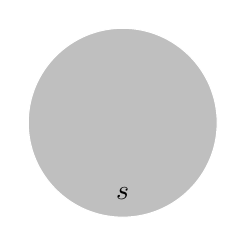
\begin{tikzpicture}
\filldraw[fill=gray!50, draw=white] (0, 0) circle (1.2);
\node at (0, -0.9) {$s$};
\end{tikzpicture}
\hspace{20pt}
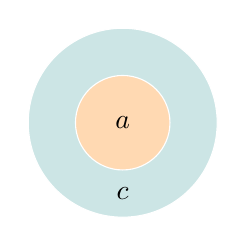
\begin{tikzpicture}
\filldraw[fill=blue!50!green!20, draw=white] (0, 0) circle (1.2);
\filldraw[fill=orange!30, draw=white] (0, 0) circle (0.6);
\node at (0, 0) {$a$};
\node at (0, -0.9) {$c$};
\end{tikzpicture}
\]



The \hask{get}/\hask{set} version of the lens can be derived from this existential form.
\begin{haskell}
toGet :: LensE s a -> (s -> a)
toGet (LensE (l, r)) = snd . l

toSet :: LensE s a -> (s -> a -> s)
toSet (LensE (l, r)) s a = r (fst (l s), a)
\end{haskell}

Notice that we don't need to know anything about the type of the residue. We take advantage of the fact that the existential lens contains both the producer and the consumer of \hask{c} and we're just mediating between the two.

It's impossible to extract a ``naked'' residue, as witnessed by the fact that the following code doesn't compile:
\begin{haskell}
getResidue :: Lens s a -> c
getResidue (Lens (l, r)) = fst . l
\end{haskell}

\subsection{Existential lens in category theory}

We can easily translate the new definition of the lens to category theory by expressing the existential type as a coend:
\[ \int^{c} \mathcal{C}(s, c \times a) \times  \mathcal{C}(c \times a, s) \]
In fact, we can generalize it to a type-changing lens, in which the focus $a$ can be replaced with a new focus of a different type $b$. Replacing $a$ with $b$ will produce a new composite object $t$:
\[
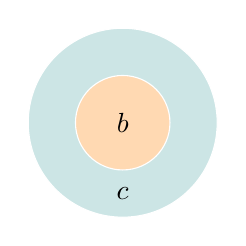
\begin{tikzpicture}
\filldraw[fill=blue!50!green!20, draw=white] (0, 0) circle (1.2);
\filldraw[fill=orange!30, draw=white] (0, 0) circle (0.6);
\node at (0, 0) {$b$};
\node at (0, -0.9) {$c$};
\end{tikzpicture}
\hspace{20pt}
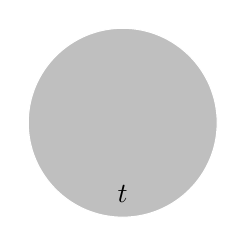
\begin{tikzpicture}
\filldraw[fill=gray!50, draw=white] (0, 0) circle (1.2);
\node at (0, -0.9) {$t$};
\end{tikzpicture}
\]

The lens is now parameterized by two pairs of objects: $\langle s, t\rangle$ for the outer ones, and $ \langle a, b \rangle$ for the inner ones. The existential residue $c$ remains hidden:
\[ \mathcal{L}\langle s, t\rangle \langle a, b \rangle = \int^{c} \mathcal{C}(s, c \times a) \times  \mathcal{C}(c \times b, t) \]
The product under the coend is the diagonal part of the profunctor that is covariant in $y$ and contravariant in $x$:
\[ \mathcal{C}(s, y \times a) \times  \mathcal{C}(x \times b, t) \]
\begin{exercise}
Show that:
\[ \mathcal{C}(s, y \times a) \times  \mathcal{C}(x \times b, t) \]
is a profunctor in $\langle x, y\rangle$.
\end{exercise}


\subsection{Type-changing lens in Haskell}
In Haskell, we can define a type-changing lens as the following existential type:
\begin{haskell}
data LensE s t a b where
  LensE :: (s -> (c, a)) -> ((c, b) -> t) -> LensE s t a b
\end{haskell}
As before, we can use it to get and set the focus:
\begin{haskell}
toGet :: LensE s t a b -> (s -> a)
toGet (LensE l r) = snd . l

toSet :: LensE s t a b -> (s -> b -> t)
toSet (LensE l r) s a = r (fst (l s), a)
\end{haskell}

The simplest example of a lens acts on a product. It can extract or replace one component of the product, treating the other as the residue. In Haskell, we'd implement it as:
\begin{haskell}
prodLens :: LensE (c, a) (c, b) a b
prodLens = LensE id id
\end{haskell}
Here, the type of the whole is the product \hask{(c, a)}. When we replace \hask{a} with \hask{b} we end up with the target type \hask{(c, b)}. Since the source and the target are already products, the two functions in the definition of the existential lens are just identities.

\subsection{Lens composition}

The main advantage of using lenses is that they compose. A composition of two lenses lets us zoom in on a subcomponent of a component. 

Suppose that we start with a lens that lets us access the focus \hask{a}  and change it to \hask{b}. This focus is part of a whole described by the source \hask{s} and the target \hask{t}. 

We also have the inner lens that can access the focus of \hask{a'}  inside the whole of \hask{a}, and replace it with \hask{b'} to produce a \hask{b}. 

We can now construct a composite lens that can access \hask{a'} and \hask{b'} inside of \hask{s} and \hask{t}. The trick is to realize that we can take, as the new residue, a product of the two residues:
\[
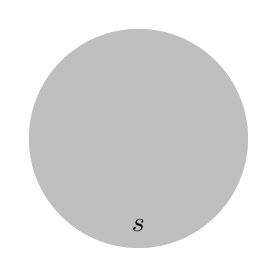
\begin{tikzpicture}
\filldraw[fill=gray!50, draw=white] (0, 0) circle (1.4);
\node at (0, -1.1) {$s$};
\end{tikzpicture}
\hspace{20pt}
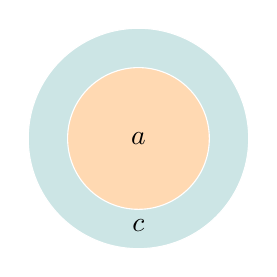
\begin{tikzpicture}
\filldraw[fill=blue!50!green!20, draw=white] (0, 0) circle (1.4);
\filldraw[fill=orange!30, draw=white] (0, 0) circle (0.9);
\node at (0, 0) {$a$};
\node at (0, -1.1) {$c$};
\end{tikzpicture}
\hspace{20pt}
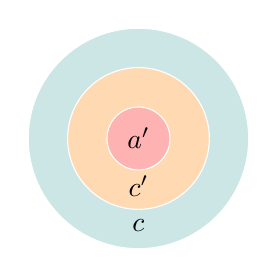
\begin{tikzpicture}
\filldraw[fill=blue!50!green!20, draw=white] (0, 0) circle (1.4);
\filldraw[fill=orange!30, draw=white] (0, 0) circle (0.9);
\filldraw[fill=red!30, draw=white] (0, 0) circle (0.4);
\node at (0, 0) {$a'$};
\node at (0, -0.6) {$c'$};
\node at (0, -1.1) {$c$};
\end{tikzpicture}
\]

\[
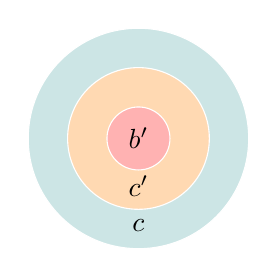
\begin{tikzpicture}
\filldraw[fill=blue!50!green!20, draw=white] (0, 0) circle (1.4);
\filldraw[fill=orange!30, draw=white] (0, 0) circle (0.9);
\filldraw[fill=red!30, draw=white] (0, 0) circle (0.4);
\node at (0, 0) {$b'$};
\node at (0, -0.6) {$c'$};
\node at (0, -1.1) {$c$};
\end{tikzpicture}
\hspace{20pt}
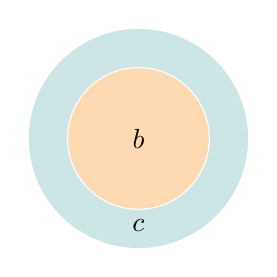
\begin{tikzpicture}
\filldraw[fill=blue!50!green!20, draw=white] (0, 0) circle (1.4);
\filldraw[fill=orange!30, draw=white] (0, 0) circle (0.9);
\node at (0, 0) {$b$};
\node at (0, -1.1) {$c$};
\end{tikzpicture}
\hspace{20pt}
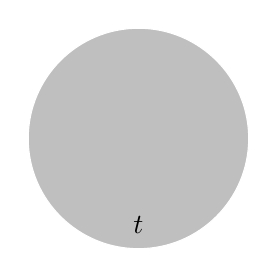
\begin{tikzpicture}
\filldraw[fill=gray!50, draw=white] (0, 0) circle (1.4);
\node at (0, -1.1) {$t$};
\end{tikzpicture}
\]



\begin{haskell}
compLens :: LensE a b a' b' -> LensE s t a b -> LensE s t a' b'
compLens (LensE l2 r2) (LensE l1 r1) = LensE l3 r3
  where l3 = assoc' . bimap id l2  . l1
        r3 = r1 . bimap id r2 . assoc
\end{haskell}
The left mapping in the new lens is given by the following composite:
\[ s \xrightarrow{l_1} (c, a)   \xrightarrow{(id, l_2)} (c, (c', a'))  \xrightarrow{assoc'} ((c, c'), a')\]
and the right mapping is given by:
\[ ((c, c'), b') \xrightarrow{assoc}  (c, (c', b')) \xrightarrow{(id, r_2)} (c, b) \xrightarrow{r_1} t \]

We have used the associativity and functoriality of the product:
\begin{haskell}
assoc :: ((c, c'), b') -> (c, (c', b'))
assoc ((c, c'), b') = (c, (c', b'))

assoc' :: (c, (c', a')) -> ((c, c'), a')
assoc' (c, (c', a')) = ((c, c'), a')

instance Bifunctor (,) where
  bimap f g (a, b) = (f a, g b)
\end{haskell}

As an example, let's compose two product lenses:
\begin{haskell}
l3 :: LensE (c, (c', a')) (c, (c', b')) a' b'
l3 = compLens prodLens prodLens
\end{haskell}
and apply it to a nested product:
\begin{haskell}
x :: (String, (Bool, Int))
x = ("Outer", (True, 42))
\end{haskell}
Our composite lens lets us not only retrieve the innermost component:
\begin{haskell}
toGet l3 x
> 42
\end{haskell}
but also replace it with a value of a different type (here, \hask{Char}):
\begin{haskell}
toSet l3 x 'z'
> ("Outer",(True,'z'))
\end{haskell}

\subsection{Category of lenses}

Since lenses can be composed, you might be wondering if there is a category in which lenses define hom-sets. 

Indeed, there is a category $\mathbf{Lens}$ whose objects are pairs of objects in $\mathcal{C}$, and arrows from $\langle s, t\rangle$ to $ \langle a, b \rangle$ are elements of  $\mathcal{L} \langle s, t\rangle \langle a, b \rangle$.

The formula for the composition of existential lenses is too complicated to be useful in practice. In the next chapter we'll see an alternative representation of lenses using Tambara modules, in which composition is just a composition of functions.

\section{Lenses and Fibrations}

There is an alternative view of lenses using the language of fiber bundles. A projection $p$ that defines a fibration can be seen as ``decomposing'' the bundle $E$ into fibers. 

In this view, $p$ plays the role of \hask{get}:
\[ p \colon E \to B \]
The base $B$ represents the type of the focus and $E$ represents the type of the composite from which that focus can be extracted.

The other part of the lens, \hask{set}, is a mapping: 
\[ q \colon E \times B \to E \]
Let's see how we can interpret it using fibrations.
\subsection{Transport law}

We interpret $q$ as ``transporting'' an element of the bundle $E$ to a new fiber. The new fiber is specified by an element of $B$.

This property of the transport is expressed by the get/set lens law, or the \emph{transport} law, that says that ``you get what you set'':
\begin{haskell}
get (set s a) = a
\end{haskell}
We say that $q(s, a)$ transports $s$ to a new fiber over $a$:

\[
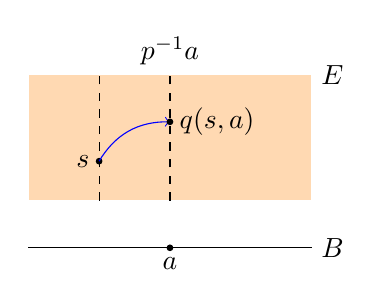
\begin{tikzpicture}

\def\yb{0}; % base
\def\yfb{0.6}; % fiber bottom
\def\yfs{1.1}; % s
\def\yfss{1.6}; % s'
\def\yft{2.2}; % fiber top

\def\dx{0.9};

\def\xbl{0};
\def\xbm{\xbl + \dx};
\def\xbmr{\xbl + 2*\dx};
\def\xbr{\xbl + 4*\dx};


\filldraw[fill=orange!30, draw=white] (\xbl, \yfb) rectangle (\xbr, \yft);

\draw (\xbl, \yb) -- (\xbr, \yb);

\draw[dashed] (\xbm, \yfb) -- (\xbm, \yft); %fiber
\draw[dashed] (\xbmr, \yfb) -- (\xbmr, \yft); %fiber

\filldraw[black] (\xbm, \yfs) circle (1 pt);
\node[left] at (\xbm, \yfs) {$s$};
\draw[blue] (\xbm, \yfs) edge[->, bend left] (\xbmr, \yfss);
\filldraw[black] (\xbmr, \yfss) circle (1 pt);
\node[right] at (\xbmr, \yfss) {$q(s, a)$};

\filldraw[black] (\xbmr, \yb) circle (1 pt);
\node[below] at (\xbmr, \yb) {$a$};

\node[above] at (\xbmr, \yft) {$p^{-1} a$};
\node[right] at (\xbr, \yb) {$B$};
\node[right] at (\xbr, \yft) {$E$};

\end{tikzpicture}
\]

We can rewrite this law in terms of $p$ and $q$:
\[ p \circ q = \pi_2 \]
where $\pi_2$ is the second projection from the product.

Equivalently, we can represent it as a commuting diagram:
\[
 \begin{tikzcd}
 E \times B
 \arrow[dd, "\varepsilon \times id"']
 \arrow[rd, "q"]
 \\
 & E
 \arrow[dl, "p"]
 \\
 B
  \end{tikzcd}
\]
Here, instead of using the projection $\pi_2$, I used a comonoidal counit $\varepsilon$:
\[ \varepsilon \colon E \to 1 \]
followed by the unit law for the product. Using a comonoid makes it easier to generalize this construction to a tensor product in a monoidal category. 

\subsection{Identity law}
Here's the set/get law or the \emph{identity} law. It says that ``nothing changes if you set what you get'':
\begin{haskell}
set s (get  s) = s
\end{haskell}
We can write it in terms of a comonoidal comultiplication:
\[ \delta \colon E \to E \times E \]
The set/get law requires the following composite to be an identity:
\[ E \xrightarrow{\delta} E \times E \xrightarrow{id \times p} E \times B \xrightarrow{q} E \]
Here's the illustration of this law in a bundle:
\[
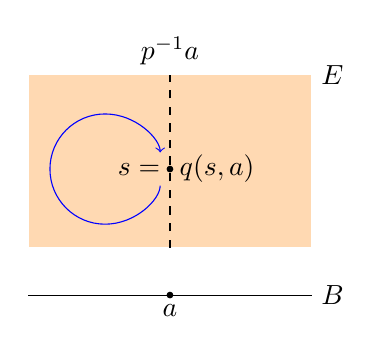
\begin{tikzpicture}

\def\yb{0}; % base
\def\yfb{0.6}; % fiber bottom
\def\yfs{1.1}; % s
\def\yfss{1.6}; % s'
\def\yft{2.8}; % fiber top

\def\dx{0.9};

\def\xbl{0};
\def\xbm{\xbl + \dx};
\def\xbmr{\xbl + 2*\dx};
\def\xbr{\xbl + 4*\dx};


\filldraw[fill=orange!30, draw=white] (\xbl, \yfb) rectangle (\xbr, \yft);

\draw (\xbl, \yb) -- (\xbr, \yb);

\draw[dashed] (\xbmr, \yfb) -- (\xbmr, \yft); %fiber

\node at (\xbmr, \yfss) (s) {};
\draw[->,shorten <=6pt,shorten >=6pt, blue](s.west)arc(360:0:0.7);
\filldraw[black] (\xbmr, \yfss) circle (1 pt);
\node[left] at (\xbmr, \yfss) {$s = $};
\node[right] at (\xbmr, \yfss) {$q(s, a)$};

\filldraw[black] (\xbmr, \yb) circle (1 pt);
\node[below] at (\xbmr, \yb) {$a$};

\node[above] at (\xbmr, \yft) {$p^{-1} a$};
\node[right] at (\xbr, \yb) {$B$};
\node[right] at (\xbr, \yft) {$E$};

\end{tikzpicture}
\]

\subsection{Composition law}

Finally, here's the set/set law, or the \emph{composition} law. It says that ``the last set wins'':
\begin{haskell}
set (set s a) a' = set s a'
\end{haskell}
and the corresponding commuting diagram:
\[
 \begin{tikzcd}
 E \times B \times B
 \arrow[d, "id \times \varepsilon \times id"']
 \arrow[rd, "q \times id"]
 \\
 E \times B
 \arrow[d, "q"']
 & E \times B
 \arrow[dl, "q "]
 \\
 E
  \end{tikzcd}
\]
Again, to get rid of the middle $B$, I used the counit rather than a projection from the product.

This is what the set/set law looks like in a bundle:
\[
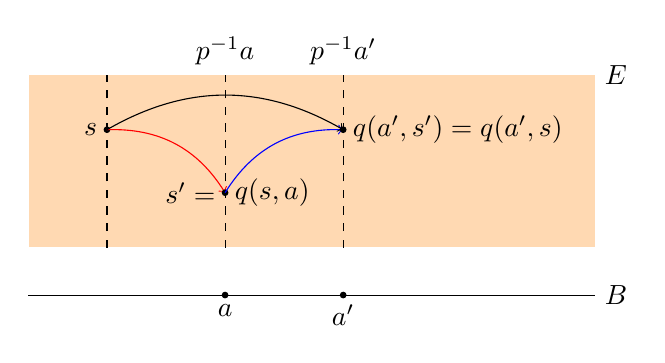
\begin{tikzpicture}

\def\yb{0}; % base
\def\yfb{0.6}; % fiber bottom
\def\yfs{1.3}; % s'
\def\yfss{2.1}; % s''
\def\yft{2.8}; % fiber top

\def\dx{1};

\def\xbl{0};
\def\xbm{\xbl + \dx};
\def\xbmr{\xbl + 2.5*\dx};
\def\xbmrr{\xbl + 4*\dx};
\def\xbr{\xbl + 7.2*\dx};


\filldraw[fill=orange!30, draw=white] (\xbl, \yfb) rectangle (\xbr, \yft);

\draw (\xbl, \yb) -- (\xbr, \yb);

\draw[dashed] (\xbm, \yfb) -- (\xbm, \yft); %fiber
\draw[dashed] (\xbmr, \yfb) -- (\xbmr, \yft); %fiber
\draw[dashed] (\xbmrr, \yfb) -- (\xbmrr, \yft); %fiber

\filldraw[black] (\xbm, \yfss) circle (1 pt);
\node[left] at (\xbm, \yfss) {$s$};

\draw[red] (\xbm, \yfss)  edge[->, bend left]  (\xbmr, \yfs);

\filldraw[black] (\xbmr, \yfs) circle (1 pt);
\node[right] at (\xbmr, \yfs) {$q(s, a)$};
\node[left] at (\xbmr, \yfs) {$s' =$};

\draw[blue] (\xbmr, \yfs) edge[->, bend left] (\xbmrr, \yfss);

\filldraw[black] (\xbmrr, \yfss) circle (1 pt);
\node[right] at (\xbmrr, \yfss) {$q(a', s') = q(a', s)$};

\draw (\xbm, \yfss) edge[->, bend left] (\xbmrr, \yfss);


\filldraw[black] (\xbmr, \yb) circle (1 pt);
\node[below] at (\xbmr, \yb) {$a$};

\filldraw[black] (\xbmrr, \yb) circle (1 pt);
\node[below] at (\xbmrr, \yb) {$a'$};

\node[above] at (\xbmr, \yft) {$p^{-1} a$};
\node[above] at (\xbmrr, \yft) {$p^{-1} a'$};
\node[right] at (\xbr, \yb) {$B$};
\node[right] at (\xbr, \yft) {$E$};

\end{tikzpicture}
\]

\subsection{Type-changing lens}

A type-changing lens generalizes transport to act between bundles. We have to define a whole family of bundles. We start with a category $\cat A$ whose objects define the types that we will use for the foci of our lens. 

We construct the set $B$ as the combined set of all elements of all focus types. $B$ is fibrated over $\cat A$---the projection $\pi$ sending an element of $B$ to its corresponding type. You may think of $B$ as the set of objects of the coslice category $1/ \cat A$.

The bundle of bundles $E$ is a set that's fibered over $B$ with the projection $p$. Since $B$ itself is fibered over $\cat A$, $E$ is transitively fibered over $\cat A$, with the composite projection $\pi \circ p$. It's this coarser fibration that splits $E$ into a family of bundles. Each of these bundles corresponds to a different type of of the composite for a given focus type. A type-changing lens will move between these bundles. 

\[
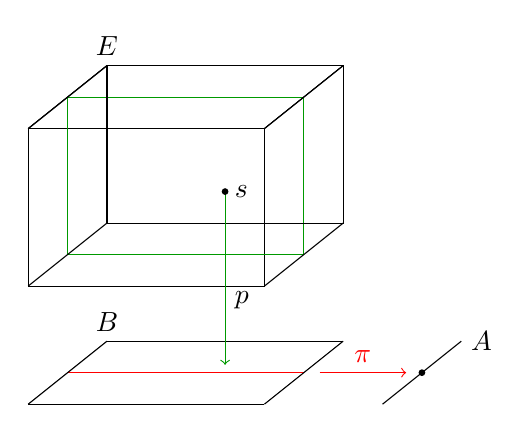
\begin{tikzpicture}
\def\xl{-3};
\def\xr{0};
\def\yb{0};
\def\yt{2};

\def\dy{0.4};
\def\dx{0.5};

\def\a{(\xl, \yb)};
\def\b{(\xr, \yb)};
\def\c{(\xl, \yt)};
\def\d {(\xr, \yt)};

% _a second plane
\def\aa{(\xl + \dx, \yb + \dy)};
\def\ba{(\xr + \dx, \yb + \dy)};
\def\ca{(\xl + \dx, \yt + \dy)};
\def\da{(\xr + \dx, \yt + \dy)};

% _b third plane
\def\ab{(\xl + 2*\dx, \yb + 2*\dy)};
\def\bb{(\xr + 2*\dx, \yb + 2*\dy)};
\def\cb{(\xl + 2*\dx, \yt + 2*\dy)};
\def\db{(\xr + 2*\dx, \yt + 2*\dy)};

% shifted walls
\def\yshift{-1.5};
\def\xshift{1.5};

% E
\draw \a rectangle \d;
\draw[draw=black!40!green] \aa rectangle \da;
\draw \ab rectangle \db;

\draw \a -- \ab;
\draw \b -- \bb;
\draw \d -- \db;
\draw \c -- \cb;

\node[above] at \cb {$E$};

% B
% rebase yb (bottom)
\def\yb{\yshift}
% rebase xr (right wall)
\def\xr{0};

\draw \a -- \b;
\draw \ab -- \bb;
\draw[red] \aa -- \ba;
% diagonal
\draw \a -- \ab;
\draw \b -- \bb;
\draw \d -- \db;
\draw \c -- \cb;
\node[above] at \ab {$B$};


% A
% rebase yb (bottom)
\def\yb{\yshift}
% rebase xr (right wall)
\def\xr{\xshift};

\draw \b -- \bb;
\node[right] at \bb {$\cat A$};
\filldraw[black] \ba circle (1 pt);

%projections

\draw[red, shorten <=0.2cm, shorten >=0.2cm, ->] (0 + \dx, \yshift + \dy) -- node[above]{$\pi$} (\xshift +\dx, \yshift + \dy);

\draw[draw=black!40!green, shorten >=0.1cm, ->] (0 - \dx, 0 + 3 * \dy) -- node[below right]{$p$} (0 - \dx, \yshift + \dy);

\node[right] at (0 - \dx, 0 + 3 * \dy) {$s$};
\filldraw[black] (0 - \dx, 0 + 3 * \dy) circle (1 pt);


\end{tikzpicture}
\]

The projection $p$ takes an element $s \in E$ and produces an element $b \in B$ whose type is given by $\pi b$. This is the generalization of \hask{get}. 

The transport $q$, which corresponds to \hask{set}, takes an element $s \in E$ and an element $b \in B$ and produces a new element $t \in E$. The important observation is that $s$ and $t$ may belong to different sub-bundles of $E$.


The transport satisfies the following laws:

The get/set law (transport):

\[ p (q (b, s)) = b \]

The set/get law (identity):

\[ q ( p (s), s) = s \]

The set/set law (composition):

\[ q (c, q (b, s)) = q (c, s) \]

\section{Important Formulas}
This is a handy (co-)end calculus cheat-sheet.
\begin{itemize}
\item Continuity of the hom-functor:
\[\cat D\left(d, \int_a P\langle a, a \rangle \right) \cong \int_a \cat D \left(d, P\langle a, a \rangle \right) \]
\item Co-continuity of the hom-functor:
\[\cat D\left( \int^a P\langle a, a \rangle , d \right) \cong \int_a \cat D \left( P\langle a, a \rangle, d \right) \]
\item Ninja Yoneda:
\[ \int_{x} \mathbf{Set} (\mathcal{C}(a, x), F x) \cong F a \]
\item Ninja co-Yoneda:
\[ \int^{x} \mathcal{C}(x, a) \times F x \cong F a \]
\item Ninja Yoneda for contravariant functors (presheaves):
\[ \int_{x} \mathbf{Set} (\mathcal{C}(x, a), G x) \cong G a \]
\item Ninja co-Yoneda for contravariant functors:
\[ \int^{x} \mathcal{C}(a, x) \times G x \cong G a \]
\item Day convolution:
\[ (F \star G) x = \int^{a, b} \cat C (a \otimes b, x) \times F a \times G b \]

\end{itemize}


\end{document}